\chapter{Methodology}\label{ch:methodology}

In this chapter we will explain the reasoning behind the choice of our research questions. 
Furthermore, in \autoref{ch:operationalization} operationalization, we formalize how we evaluate these research questions. 
We then proceed in \autoref{sec:ground-truth}, to establish a ground truth, which tests both white-box analysis and black-box analysis in 
different scenarios.

\section{Operationalization}\label{ch:operationalization}

In this section, we explain the reasoning behind picking \hyperref[researchQuestions]{research questions \ref*{researchQuestions}} 
and formalize how we evaluate them. The focus point of this thesis is to identify if we can use both the white-box and black-box models 
to evaluate configurable software systems. In the following, we will reintroduce the research questions and explain what the question aims to achieve:\\

\noindent \textbf{RQ1}: How accurately do white-box and black-box models detect feature and feature interactions? \\

One of the main points we research in this thesis is how accurately we can identify features and especially interactions between features. 
We design multiple small configurable systems in the ground truth section to investigate this. 
We investigate this using our ground truth because, in these systems, 
we are fully aware of how much time we should spend in each feature or feature interaction. 
Therefore, we quantify the difference between the predicted and true influence by calculating for each feature and 
feature interaction the absolute percentage error (APE) and afterward the accuracy of the whole model by calculating the mean absolute percentage error 
(MAPE)~\cite{mape}. %Maybe reference

We calculate the APE and MAPE as follows:

\begin{align}
    \text{APE}(c) &= \frac{\lvert \Pi_{true}(c(o_j)) - \widehat{\Pi}(c(o_j))\rvert}{\Pi_{true}(c(o_j))} \label{equ:APE} \\ \nonumber \\
    \text{MAPE}(C) &= \frac{\sum_{c \in C} \text{APE}(c)}{\lvert C \rvert} \label{equ:mape}
\end{align}

Note that $\Pi_{true}(c(o_j))$ is the true influence of the feature $o_j$ that we obtain from the baseline of our ground truth 
and $\widehat{\Pi}(c(o_j))$ the influence predicted by the {\perfInfluenceModel}s we build.
The closer MAPE is to $0$, the better the prediction since, 
for the MAPE to be $0$ the predicted influence of each feature needs to be the same as the true influence; 
in this case, our performance would be completely accurate. \\

\noindent \textbf{RQ2}: Do performance models created by our white-box and black-box attribute the same influence to each feature?\\

In this research question, we investigate whether the {\perfInfluenceModel}s build-out of the white-box and black-box analyses' data agree, 
meaning they predict the same influence for each feature. 
Compared to RQ1, we do not measure if the predictions are accurate regarding the true influence but if both analyses produce similar results. 
For this, we again use APE and MAPE. However, we need to adjust the formula as follows:

\begin{align}
    \text{APE}(c) &= \frac{\lvert\Pi_{WB}(c(o_j)) - \Pi_{BB}(c(o_j))\rvert}{\Pi_{WB}(c(o_j))} \label{equ:APE} \\ \nonumber \\
    \text{MAPE}(C) &= \frac{\sum_{c \in C} \text{APE}(c)}{\lvert C \rvert} \label{equ:mape}
\end{align}

Here we quantify the difference between the predictions of white-box $\Pi_{WB}$ and black-box $\Pi{BB}$ for each feature $o_j$, 
the closer the MAPE score is to $0$ the more similar our {\perfInfluenceModel}s are.\\

\noindent \textbf{RQ3}: What are the reasons for similarities or differences between performance models?\\

In RQ2, we investigate how similar both {\perfInfluenceModel}s are with each other. 
However, we are also interested in why both models are the same or different, but compared to RQ1 and RQ2, these reasons are not quantifiable. 
As such, we use our knowledge of both white-box and black-box to try and identify the reasons for this. Reasons for a difference could be 
that the configurable system contains a large amount of multicollinearity; therefore, the black-box analysis estimator is suboptimal. 
For the white-box analysis, the reason might be that the taint analysis is unable to follow feature variables throughout the system.

\section{Collecting Data}\label{ch:collect-data}
After deciding which features interest us, we turn to how we collect our data, which we can use to create the {\perfInfluenceModel}s.

The non-functional property that we decide to analyze is performance because it is one metric of high interest for stakeholders. 
It is also an easily quantifiable metric that reflects the changes to the system if a feature with a significant influence is selected.

Every measurement is subject to noise, which influences the measured performance during the execution of the system. 
To reduce this noise, we measure each configuration 30 times and take the mean of the time spent as values to build the {\perfInfluenceModel}s~\cite{SampleSize}.

To collect the data by using the VaRA Tool Suite in which we define an experiment for each project, we analyze. 
In this experiment, we specify how we want to analyze the project and in which way. For our white-box analysis, 
we write an experiment that specifies that we want to use VaRA to instrument our code so that during execution, 
all trace events can be tracked and written into the TEF report file. For our black-box analysis, 
we wrap the command we want to measure with the Linux time command and write the time spent into a different report. 
Each measurement is done sequentially and on the same machine. 

\subsection*{Noteworthy tools}
During both the experiments we use different frameworks and libarys, we will mention the noteworthy ones here.

Besides VaRA Tool Suite we also use plumbum\footnote{Visited at 02.04.2023 https://plumbum.readthedocs.io/en/latest/}
%SKLearn 
%statsmodels.stats.outliers_influence import variance_inflation_factor
\section{Ground Truth}\label{sec:ground-truth}
In this section, we introduce a ground truth to establish that both black-box analysis from \autoref{ch:Blackbox} 
and white-box analysis from \autoref{ch:Whitebox} can analyze simple, configurable systems and identify weaknesses. 

To do so, we design multiple configurable systems that test both analyses in different scenarios. 
Afterward, we evaluate them using the research questions from \autoref{ch:operationalization}. 
Since we design these systems ourselves, we have a baseline that we use to build a {\perfInfluenceModel} for each system manually. 
We design all the systems with different focuses in mind, such as a system that includes multicollinearity, 
to see to what extent they influence the analyses. 
We investigate all the changes to \emph{Simple interaction} system independent of another to pinpoint the reason if the analyses
are inaccurate, therefore, none of the changes are persistent.


\paragraph{Simple interaction}\label{ground-truth:Simple}
For our first system, we use the code from our previous example in \autoref{lst:performanceExample} and provide an additional feature model 
of the system in \autoref{fig:feature_abcd}. 
We use this system as our base system, which we extend for each scenario; therefore it is the simplest one, 
only containing some interactions and no constraints.

\begin{figure}[h]
    \centering
    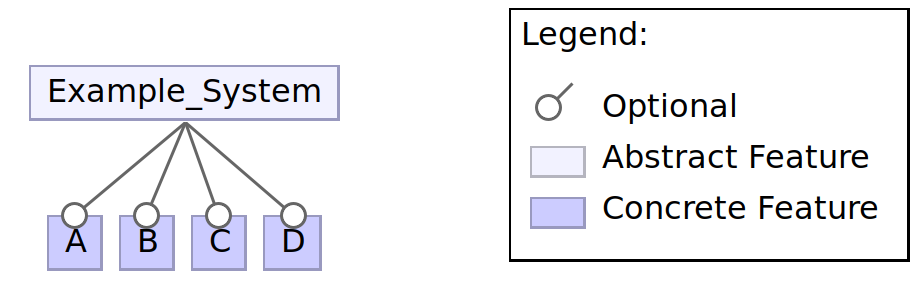
\includegraphics[scale=0.25]{gfx/Feature_ABCD.png}
    \caption{Feature model of \autoref{lst:performanceExample}.}
    \label{fig:feature_abcd}
\end{figure}


\paragraph{Else clause}
The first modification we do is adding an \emph{else clause} to the if statement of feature \emph{A} in \autorefLine{line:feature_A_statement}. 
We encode this as follows:

\begin{minipage}{\linewidth}
    \begin{lstlisting}[language=C++,label={lst:else_case},escapechar=|]
if(A)
    fpcsc::sleep_for_secs(1); 
else
    fpcsc::sleep_for_secs(2);
    \end{lstlisting}
    \end{minipage}

We expect the white-box analysis to attribute the time spent in the else case to feature \emph{A} 
since it is a part of the feature region of feature \emph{A}. 
In contrast, 
the black-box analysis cannot differentiate between the else clause that is executed when feature \emph{A} is unselected and the time spent in \emph{Base}.

\paragraph{Function}\label{ground-truth:Function}
The next modification of our basic system is adding a function to the system in which we spent time. 
In \autorefLine{line:feature_A} we call the function \emph{waste\_time(1)} instead of \emph{fpcsc::sleep\_for\_secs(1)}, in which we spent time a second.

\begin{minipage}{\linewidth}
\begin{lstlisting}[language=C++,label={lst:function},escapechar=|]
void waste_time(int duration){
    fpcsc::sleep_for_secs(duration);
    }
\end{lstlisting}
\end{minipage}

This modification should not affect the black-box analysis since the overall time spent in each feature does not change. 
We would like to see if the white-box analysis can still attribute the time correctly to the feature.

\paragraph{Multicollinearity}\label{ground-truth:Multicollinearity}
Instead of modifying the system's code, we add a restriction to the feature model of \autoref{fig:feature_abcd}. 
We change feature \emph{B} from optional to mandatory. This introduces multicollinearity into the system. 
The white-box analysis should still be able to identify correctly the time spent in \emph{Base} and feature \emph{B}, 
while the black-box analysis should distribute the time spent between \emph{Base} and \emph{B} differently.

\paragraph{Shared Feature Variable}\label{ground-truth:Shared}
We now add an optional feature \emph{E} to the system. 
However, instead of encoding it like the previous features by specifying a separate variable, 
we modify the feature variable \emph{D} in \autorefLine{line:feature_declatation} to a \emph{string de = "00"} 
for which the first character represents feature \emph{D} and the second character \emph{E}. If either is selected, 
we assign the character for that feature \emph{"1"}. We add another if statement to spend time when \emph{E} is selected and encode this as follows:

\begin{minipage}{\linewidth}
\begin{lstlisting}[language=C++,label={lst:shared},escapechar=|]
std::string de = "00";

if(de[0] == '1')
    fpcsc::sleep_for_secs(2);

if(de[1] == '1')
    fpcsc::sleep_for_secs(1);
\end{lstlisting}
\end{minipage}

We expect the black-box analysis to work still as intended. 
However, the white-box analysis to be inaccurate since both features \emph{D} and \emph{E} share the same feature variable. 
Each feature region of \emph{D} or \emph{E} should now be influenced by the feature interaction \emph{\{D, E\}}.